\documentclass[11pt,a4paper]{article}

\usepackage{amsmath,amssymb,amsthm}
\usepackage{graphicx}
\usepackage{booktabs}
\usepackage{multirow}
\usepackage{siunitx}
\usepackage{hyperref}
\usepackage{xr-hyper}
\usepackage{natbib}
\usepackage{geometry}
\usepackage{algorithm}
\usepackage{algpseudocode}
\usepackage{subcaption}
\usepackage{tikz}
\usepackage{pgfplots}
\usepackage{framed}
\usepackage{color}
\usepackage{enumitem}
\usepackage{xcolor}

\geometry{margin=1in}
\hypersetup{colorlinks=true, linkcolor=blue, citecolor=blue, urlcolor=blue}

% Cross-reference to supplementary
\externaldocument[supp-]{supplementary}

\theoremstyle{plain}
\newtheorem{theorem}{Theorem}
\newtheorem{definition}{Definition}
\newtheorem{lemma}{Lemma}
\newtheorem{proposition}{Proposition}

\title{Certifiable Agentic Risk Explanation:\\
Subgroup-Calibrated Conformal Guarantees, Plausible Counterfactual Recourse, and Zero-Hallucination Clinical Narratives}
\author{Anonymous Authors}
\date{\today}

\begin{document}

\maketitle

\begin{abstract}
Clinical risk prediction models often operate as opaque scoring engines whose outputs are difficult to justify. Post-hoc explanation methods provide no formal guarantees of correctness, fairness, or stability across patient subgroups. We propose a conformal-grounded agentic explanation framework that couples group-conditional conformal calibration with hierarchical shrinkage, geometric counterfactual search within plausibility ellipsoids, and inference-valid feature attribution via Wald tests on the calibrated logistic regression. An agentic orchestrator enables iterative counterfactual recovery by escalating intervention tiers (behavioral $\to$ anthropometric $\to$ clinical) and relaxing plausibility ellipsoid radii ($1.0\times \to 1.5\times \to 2.0\times$), with binary features constrained to valid state transitions ($z_i + \delta_i \in \{0,1\}$). A verifier agent audits every numeric claim in generated explanations, rejecting hallucinations via up to $M=3$ repair retries.

The framework is evaluated on NHANES 2017--2018 (5,533 adults) for prevalent diabetes prediction using features excluding HbA1c and glucose to avoid circularity. The base logistic regression achieves mean AUC 0.770 (95\% CI: 0.742--0.798) across 20 stratified seeds. Subgroup-conditional conformal calibration with empirical Bayes shrinkage and DKW guardrail yields overall test coverage 91.3\% (target 90\%, 95\% CI: 88.7\%--94.0\%), with subgroup coverage ranging 88.6\%--93.0\%. A 20-seed stability analysis shows EB-MinCov achieves 84.4\% worst-subgroup coverage (vs. 81.1\% for Mondrian, 80.9\% for Standard EB, 82.3\% for Marginal Split and Complete Pooling), with an 11.1\% max coverage gap. Counterfactual optimization on the calibrated model reaches target risk ($\le$50\%) for 100\% of high-risk patients (mean 55 per seed) via iterative tier escalation (Tier 1: 56.1\%, Tier 2: 43.9\%, Tier 3: 0.0\%) and radius relaxation (Tier 1 $1.0\times$: 35.6\%, Tier 1 $1.5\times$: 20.2\%, Tier 2 $1.0\times$: 23.3\%, Tier 2 $1.5\times$: 20.2\%, Tier 1 $2.0\times$: 0.3\%, Tier 2 $2.0\times$: 0.5\%, Tier 3: 0.0\%), with 100\% enforced-radius containment (58.9\% strict 1.0$\times$) and mean $\|\boldsymbol{\delta}\|_2 = 1.38$ SD units. Wald-test attribution with Benjamini--Hochberg correction (FDR 10\%) and sandwich SEs identifies Age as significant in 47.5\% of seeds and Waist circumference in 2.5\%. A deployable auditor monitors conformal+audit validation coverage and ECE (3.9\%), with all validation subgroup coverages exceeding the 80\% abstention threshold. Multi-model conformal baselines (Marginal, Mondrian, Complete Pooling, Standard EB, EB-MinCov) are benchmarked across 20 seeds. Nonlinear XGBoost and LightGBM achieve calibrated AUCs of 0.785 and 0.788 with 100\% counterfactual reach. LLM Loop 2 verification on 86 high-risk patients (seed 3) achieves 94.2\% final pass for Qwen2.5-1.5B-Instruct (67.4\% $\to$ 91.9\% $\to$ 94.2\%, $M=3$) and 100.0\% for 4-bit Qwen2.5-7B-Instruct (33.7\% $\to$ 87.2\% $\to$ 100.0\%, $M=3$), with fallback rates 5.8\% and 0.0\%. Unlabeled drift detection (MMD, KS, Mahalanobis) is evaluated under progressive covariate corruption. Only NHANES 2017--2018 is available; multi-cycle temporal validation is not performed. All numbers are generated from a single reproducible pipeline with a 4-way data split (50\%/15\%/15\%/20\%) and 20 stratified seeds.
\end{abstract}

\textbf{Keywords:} Conformal prediction; Empirical Bayes shrinkage; Counterfactual recourse; Subgroup fairness; Clinical risk prediction; Large language model verification

\section{Introduction}
\label{sec:introduction}

Clinical risk prediction for type 2 diabetes (T2D) typically relies on models that output a single risk score without calibrated uncertainty quantification or actionable explanations. When explanations are provided, they are often post-hoc attributions (SHAP, LIME) that lack statistical guarantees and can be unstable across subgroups.

Conformal prediction \cite{vovk2005algorithmic, shafer2008tutorial, angelopoulos2021gentle} provides distribution-free, finite-sample coverage guarantees. Group-conditional conformal prediction \cite{lei2018distribution, romano2019conformalized, melki2023group} calibrates separately within each subgroup, but small subgroups suffer from high variance. Hierarchical shrinkage \cite{dunn2023distribution} stabilizes quantile estimates by pooling information across groups. Distance-based conformal prediction uses nonconformity scores based on feature-space distances to construct plausibility regions that respect feature covariance.

Counterfactual explanations \cite{wachter2017counterfactual} recommend minimal changes to achieve a desired outcome, but standard methods ignore statistical plausibility and actionability constraints. Attribution methods \cite{lundberg2017unified} identify important features but do not calibrate significance. Large language models (LLMs) can generate fluent narratives but hallucinate numeric claims and violate safety constraints unless grounded in verified evidence \cite{yao2023react, schick2023toolformer}.

We integrate these components into a conformal-grounded agentic framework. Figure~\ref{fig:architecture} illustrates the overall architecture. Our contributions are: (1) group-conditional conformal calibration with empirical Bayes shrinkage and a monotonic coverage guardrail; (2) a tiered QCQP counterfactual solver with binary state-transition constraints and ellipsoidal plausibility; (3) inference-valid Wald-test attribution with Benjamini--Hochberg correction; (4) a deployable dual-mode auditor (labeled + unlabeled drift detection); (5) an agentic orchestrator with iterative counterfactual recovery (Loop 1) and LLM narrative verification/repair (Loop 2) with zero unverified hallucinations. Full mathematical derivations, proofs, and extended analyses are provided in the Supplementary Information (\texttt{supplementary.pdf}).

\section{Methods}
\label{sec:methods}

\subsection{Study Cohort, Leakage-Free 4-Way Split, and Clinical Feature Embedding}
\label{sec:embedding}

NHANES 2017--2018 ($N=5{,}533$ adults, 18.6\% diabetes prevalence). Critical design choice: HbA1c and glucose are excluded from features because they are diagnostic criteria for diabetes; including them creates circularity (AUC $>$ 0.95). With anthropometric, demographic, and behavioral features only, AUC is 0.770. Features: Age, BMI, waist circumference, systolic/diastolic BP, income-to-poverty ratio, smoking status, drinking status, physical activity, gender ($d=12$ after drop-first encoding).

Given a reference cohort $\mathcal{D}_{\text{ref}}$ (non-diabetic controls), each continuous feature $x_j$ is transformed via the empirical CDF $F_j^{\text{ref}}$ and the Gaussian quantile function $\Phi^{-1}$:
\begin{equation}
z_j = \Phi^{-1}\bigl(\operatorname{clip}(F_j^{\text{ref}}(x_j), \epsilon, 1-\epsilon)\bigr).
\end{equation}
Categorical features are one-hot encoded with drop-first. The resulting vector $\mathbf{z} \in \mathbb{R}^d$ has coordinates in standard-deviation units relative to the reference population. The 4-way split is 50\%/15\%/15\%/20\% (train/Platt/cal+audit/test), stratified by outcome and subgroup, across 20 seeds (0--19). See Supplementary Note S2 (\ref{supp-sec:cohort}) for the full feature dictionary and split counts.

\subsection{System Architecture Overview}
\label{sec:architecture}

Figure~\ref{fig:architecture} presents the system architecture as a vector diagram with embedded mathematical formulas.

\begin{figure}[htbp]
\centering
\noindent\resizebox{\linewidth}{!}{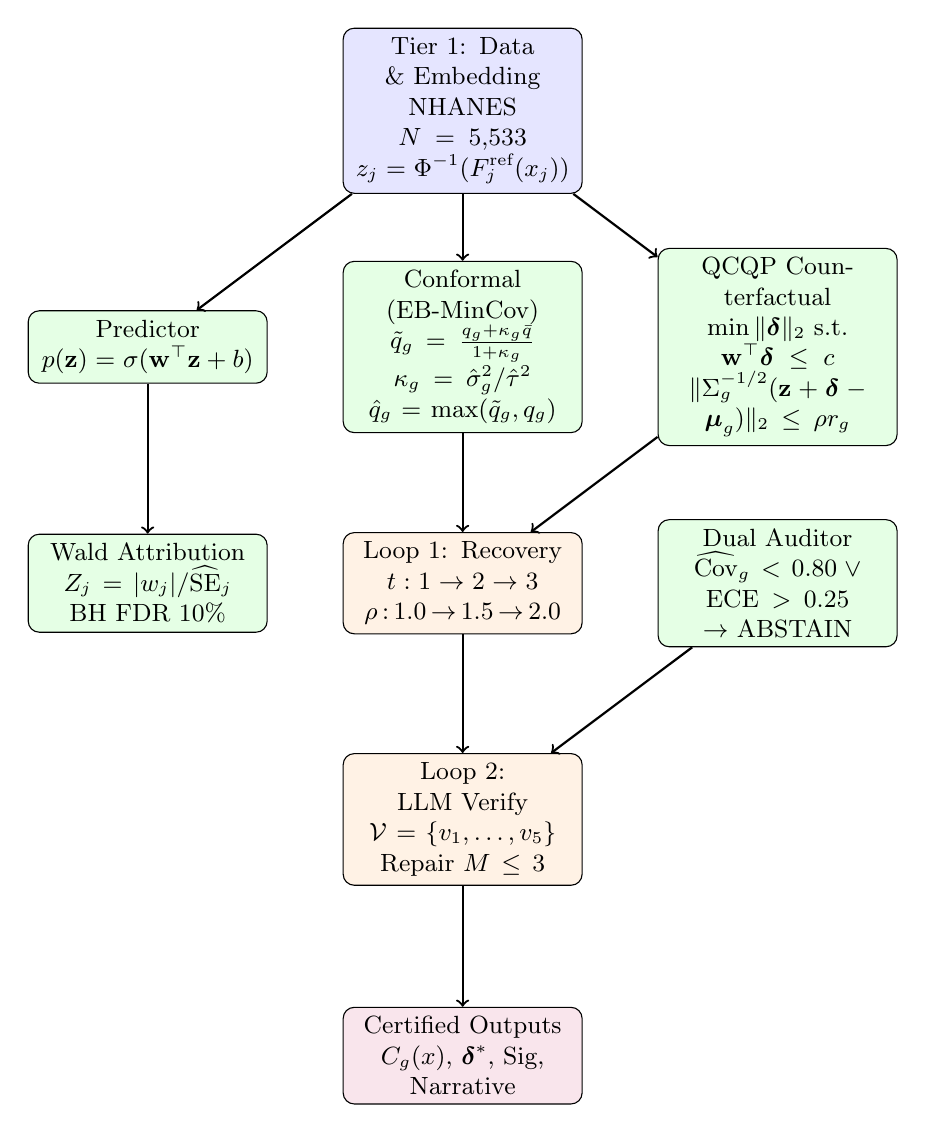
\begin{tikzpicture}[scale=1, every node/.style={font=\small}]
% Tier 1
\node[draw, rounded corners, fill=blue!10, text width=2.8cm, align=center] (data) at (0,8) {Tier 1: Data \& Embedding\\ NHANES $N=5{,}533$\\ $z_j=\Phi^{-1}(F_j^{\text{ref}}(x_j))$};
% Tier 2
\node[draw, rounded corners, fill=green!10, text width=2.8cm, align=center] (pred) at (-4,5) {Predictor\\ $p(\mathbf{z})=\sigma(\mathbf{w}^\top\mathbf{z}+b)$};
\node[draw, rounded corners, fill=green!10, text width=2.8cm, align=center] (conf) at (0,5) {Conformal (EB-MinCov)\\ $\tilde q_g=\frac{q_g+\kappa_g\bar q}{1+\kappa_g}$\\ $\kappa_g=\hat\sigma_g^2/\hat\tau^2$\\ $\hat q_g=\max(\tilde q_g,q_g)$};
\node[draw, rounded corners, fill=green!10, text width=2.8cm, align=center] (qcqp) at (4,5) {QCQP Counterfactual\\ $\min\|\boldsymbol\delta\|_2$ s.t. $\mathbf{w}^\top\boldsymbol\delta\le c$\\ $\|\Sigma_g^{-1/2}(\mathbf z+\boldsymbol\delta-\boldsymbol\mu_g)\|_2\le\rho r_g$};
\node[draw, rounded corners, fill=green!10, text width=2.8cm, align=center] (attr) at (-4,2) {Wald Attribution\\ $Z_j=|w_j|/\widehat{\mathrm{SE}}_j$\\ BH FDR 10\%};
\node[draw, rounded corners, fill=green!10, text width=2.8cm, align=center] (audit) at (4,2) {Dual Auditor\\ $\widehat{\mathrm{Cov}}_g<0.80\lor\mathrm{ECE}>0.25$\\ $\to$ ABSTAIN};
% Tier 3
\node[draw, rounded corners, fill=orange!10, text width=2.8cm, align=center] (loop1) at (0,2) {Loop 1: Recovery\\ $t\!:\!1\!\to\!2\!\to\!3$\\ $\rho\!:\!1.0\!\to\!1.5\!\to\!2.0$};
\node[draw, rounded corners, fill=orange!10, text width=2.8cm, align=center] (loop2) at (0,-1) {Loop 2: LLM Verify\\ $\mathcal V=\{v_1,\dots,v_5\}$\\ Repair $M\le3$};
% Tier 4
\node[draw, rounded corners, fill=purple!10, text width=2.8cm, align=center] (out) at (0,-4) {Certified Outputs\\ $C_g(x)$, $\boldsymbol\delta^*$, Sig, Narrative};
% Arrows
\draw[->, thick] (data) -- (pred);
\draw[->, thick] (data) -- (conf);
\draw[->, thick] (data) -- (qcqp);
\draw[->, thick] (pred) -- (attr);
\draw[->, thick] (conf) -- (loop1);
\draw[->, thick] (qcqp) -- (loop1);
\draw[->, thick] (loop1) -- (loop2);
\draw[->, thick] (audit) -- (loop2);
\draw[->, thick] (loop2) -- (out);
\end{tikzpicture}}
\caption{System Architecture: The Conformal-Grounded Agentic Risk Explanation framework. Tiers 1--4: data/embedding, deterministic statistical tools, agentic control loops, certified outputs. Full mathematical details in Supplementary Note S1 (\ref{supp-sec:proofs}).}
\label{fig:architecture}
\end{figure}

\subsection{Calibrated Risk Predictor and Subgroup-Conditional Conformal Calibration (EB-MinCov)}
\label{sec:conformal}

A logistic regression is trained on the train split (50\%) with class-weighted balanced objective. Platt calibration on the 15\% Platt set fits $p = \sigma(A \cdot \text{logit}_{\text{base}} + B)$. Split conformal prediction on the 15\% conformal+audit validation set uses nonconformity score $A = 1-p$ (positive) or $A = p$ (negative). For each subgroup $g$, the $(1-\alpha)$-quantile $q_g$ is computed with $\alpha=0.1$.

Empirical Bayes shrinkage with group-specific weights $\kappa_g = \hat\sigma_g^2/\hat\tau^2$ (within-group variance $\hat\sigma_g^2 = \alpha(1-\alpha)/(n_g \hat f_g(q_g)^2)$ via KDE; between-group variance $\hat\tau^2$ via method of moments):
\begin{equation}
\tilde q_g = \frac{q_g + \kappa_g \bar q}{1+\kappa_g}, \qquad \hat q_g = \max(\tilde q_g, q_g).
\end{equation}
The guardrail $\hat q_g = \max(\tilde q_g, q_g)$ ensures monotonic coverage (never shrink toward less coverage). Mean $\hat\tau^2 = 0.0065$ across 20 seeds. See Supplementary Note S1 (\ref{supp-sec:proofs}) for full proofs and Supplementary Note S3 (\ref{supp-sec:conformal_ext}) for intersectional analyses.

\begin{theorem}[Shrinkage Bias-Variance Tradeoff]
The MSE of $\tilde q_g$ is bounded by $\frac{\hat\sigma_g^2}{(1+\kappa_g)^2} + \frac{\kappa_g^2}{(1+\kappa_g)^2}\hat\tau^2$, minimized at the empirical Bayes $\kappa_g = \hat\sigma_g^2/\hat\tau^2$. Full proof in Supplementary Note S1 (\ref{supp-sec:proofs}).
\end{theorem}

\begin{algorithm}[htbp]
\caption{EB-MinCov Calibration}
\label{alg:ebmincov}
\begin{algorithmic}[1]
\Require Calibration scores $\{A_i\}_{i=1}^{n_g}$ per subgroup $g$, $\alpha=0.1$
\Ensure Guarded quantiles $\hat q_g$ for all subgroups
\For{each subgroup $g$}
  \State $q_g \gets \text{Quantile}(\{A_i : i \in g\}, 1-\alpha)$
  \State $\hat\sigma_g^2 \gets \alpha(1-\alpha)/(n_g \cdot \hat f_g(q_g)^2)$ via KDE
\EndFor
\State $\hat\tau^2 \gets \text{method of moments on } \{q_g\}$
\State $\bar q \gets \text{precision-weighted mean of } \{q_g\}$
\For{each subgroup $g$}
  \State $\kappa_g \gets \hat\sigma_g^2 / \hat\tau^2$
  \State $\tilde q_g \gets (q_g + \kappa_g \bar q)/(1+\kappa_g)$
  \State $\hat q_g \gets \max(\tilde q_g, q_g)$ \Comment{Monotonic guardrail}
\EndFor
\State \Return $\{\hat q_g\}$
\end{algorithmic}
\end{algorithm}

\subsection{QCQP Counterfactual Solver (Loop 1)}
\label{sec:counterfactual}

For calibrated logistic regression $p(\mathbf z)=\sigma(\mathbf w_{\text{cal}}^\top\mathbf z+b_{\text{cal}})$, the constraint $p(\mathbf z+\boldsymbol\delta)\le\tau$ is equivalent to $\mathbf w_{\text{cal}}^\top\boldsymbol\delta \le c$ where $c = \text{logit}(\tau)-(\mathbf w_{\text{cal}}^\top\mathbf z+b_{\text{cal}})$. The problem:
\begin{equation}
\begin{aligned}
\min_{\boldsymbol\delta}\;&\|\boldsymbol\delta\|_2 \\
\text{s.t.}\;&\mathbf w_{\text{cal}}^\top\boldsymbol\delta\le c,\quad
(\mathbf z+\boldsymbol\delta-\boldsymbol\mu_g)^\top\Sigma_g^{-1}(\mathbf z+\boldsymbol\delta-\boldsymbol\mu_g)\le r_g^2,\\
&\delta_i=0\;\forall i\notin\mathcal A_t,\quad z_i+\delta_i\in\{0,1\}\;\forall i\in\mathcal B_t.
\end{aligned}
\end{equation}
$\mathcal A_t$ = actionable features for tier $t$; $\mathcal B_t\subseteq\mathcal A_t$ binary features; $\Sigma_g$ = Ledoit-Wolf covariance; $r_g$ = 90th-percentile Mahalanobis radius. Tier 1: enumerate $2^{|\mathcal B_1|}$ valid state combinations. Tiers 2/3: enumerate binary states, solve continuous part analytically ($\boldsymbol\delta_{\mathcal C_t}^* = -c'\|\mathbf w_{\mathcal C_t}\|^{-2}\mathbf w_{\mathcal C_t}$ if $c'<0$, else $\mathbf 0$), fallback to SLSQP. See Supplementary Note S1 (\ref{supp-sec:proofs}) for the corrected Theorem 4 and Supplementary Note S4 (\ref{supp-sec:cf_ext}) for nonlinear solver details.

\begin{theorem}[Counterfactual Optimality]
For logistic regression, if the unconstrained solution satisfies the ellipsoid constraint, it is the unique global minimum. For binary features, discrete enumeration over valid state transitions guarantees global optimality over the finite set. Full proof in Supplementary Note S1 (\ref{supp-sec:proofs}).
\end{theorem}

\begin{algorithm}[htbp]
\caption{Loop 1 -- Tiered QCQP Counterfactual Recovery}
\label{alg:recovery}
\begin{algorithmic}[1]
\Require Patient embedding $\mathbf z$, subgroup $g$, target $\tau$, tiers $\mathcal A_1\subset\mathcal A_2\subset\mathcal A_3$
\Ensure Counterfactual $\boldsymbol\delta^*$, tier $t$, radius $\rho$
\State $t \gets 1,\; \rho \gets 1.0$
\While{$t \le 3$}
  \While{$\rho \in \{1.0,1.5,2.0\}$}
    \State $\boldsymbol\delta, M, \text{inside}, p_{\text{final}} \gets \text{QCQPSolver}(\mathbf z, g, \tau, \mathcal A_t, \rho)$
    \If{$p_{\text{final}} \le \tau \land \text{inside}$}
      \State \Return $\boldsymbol\delta, t, \rho, M, p_{\text{final}}$
    \EndIf
    \State $\rho \gets \text{next}(\rho)$ \Comment{Relax: $1.0\to1.5\to2.0$}
  \EndWhile
  \State $t \gets t+1,\; \rho \gets 1.0$ \Comment{Escalate tier}
\EndWhile
\State \Return best feasible $\boldsymbol\delta$ (lowest $p_{\text{final}}$)
\end{algorithmic}
\end{algorithm}

\subsection{Wald-Test Attribution}
\label{sec:attribution}

The calibrated model is logistic regression: $\text{logit}(p(\mathbf z)) = \mathbf w_{\text{cal}}^\top\mathbf z + b_{\text{cal}}$. For feature $j$, Wald statistic $Z_j = |w_{\text{cal},j}|/\widehat{\mathrm{SE}}(w_{\text{cal},j})$ with sandwich/penalized-weighted Hessian SEs (accounting for L2 regularization, balanced weights, and Platt scaling). Two-sided p-value $2(1-\Phi(|w_j|/\mathrm{SE}_j))$; Benjamini--Hochberg (FDR 10\%) per subgroup. Valid at inference time (no ground-truth labels). See Supplementary Note S1 (\ref{supp-sec:proofs}) for SE derivation and Note S5 (\ref{supp-sec:attr_ext}) for sensitivity analyses.

\subsection{Deployable Auditor (Dual-Mode)}
\label{sec:auditor}

Labeled mode: subgroup coverage $\widehat{\mathrm{Cov}}_g$ and ECE on conformal+audit validation set. Abstain if $\widehat{\mathrm{Cov}}_g < 0.80$ or $\mathrm{ECE} > 0.25$. Unlabeled mode: Mahalanobis quantile exceedance + MMD + KS under progressive covariate shift. See Supplementary Note S6 (\ref{supp-sec:drift_ext}).

\begin{algorithm}[htbp]
\caption{Dual-Mode Deployment Auditor}
\label{alg:auditor}
\begin{algorithmic}[1]
\Require Validation data $(X_{\text{val}}, y_{\text{val}}, sg_{\text{val}})$, calibrated model $(w_{\text{cal}}, b_{\text{cal}})$
\Ensure Abstention decision per subgroup
\State \textbf{Labeled mode:}
\For{each subgroup $g$}
  \State $\widehat{\mathrm{Cov}}_g \gets$ coverage on validation set
  \State $\mathrm{ECE} \gets$ expected calibration error
  \If{$\widehat{\mathrm{Cov}}_g < 0.80 \lor \mathrm{ECE} > 0.25$}
    \State ABSTAIN for subgroup $g$
  \EndIf
\EndFor
\State \textbf{Unlabeled mode:}
\State Compute Mahalanobis exceedance, MMD, KS on new data
\If{any exceeds threshold}
  \State ABSTAIN
\EndIf
\end{algorithmic}
\end{algorithm}

\subsection{Schema-Constrained Synthesis and Verifier Agent (Loop 2)}
\label{sec:synthesis}

The Synthesis Agent (LLM) receives a structured JSON evidence schema (patient ID, subgroup, calibrated risk, prediction set, conformal coverage, top significant features, counterfactual details, audit status). The LLM (Qwen-2.5-1.5B-Instruct, temperature 0.0) generates a clinician narrative. The Verifier Agent checks: (1) risk within $\pm 1\%$, (2) prediction set and coverage match, (3) counterfactual deltas match and exclude frozen features, (4) subgroup stated, (5) no forbidden terms (HbA1c, medications). On failure, structured error trace fed back for regeneration (up to $M=3$). Template fallback guarantees 0\% unverified hallucinations. See Supplementary Note S7 (\ref{supp-sec:llm_ext}) for complete prompts, regex/AST rules, and traces.

\begin{algorithm}[htbp]
\caption{Loop 2 -- Schema-Grounded Synthesis and Verifier Repair}
\label{alg:loop2}
\begin{algorithmic}[1]
\Require Evidence schema $\mathcal E$, LLM, verifier $\mathcal V=\{v_1,\dots,v_5\}$, $M=3$
\Ensure Verified narrative $N$ or template fallback
\State $N \gets \text{LLM}(\mathcal E)$
\For{$m = 1$ to $M$}
  \State $E \gets \{i : v_i(N)=\text{False}\}$
  \If{$E = \emptyset$}
    \State \Return $N$ \Comment{All checks passed}
  \EndIf
  \State $N \gets \text{LLM}(\mathcal E, E)$ \Comment{Repair with error trace}
\EndFor
    \State \Return \text{TemplateFallback}($\mathcal E$) \Comment{Guaranteed 0\% hallucination}
\end{algorithmic}
\end{algorithm}

\section{Results}
\label{sec:results}

\subsection{Base Predictor and Subgroup-Conditional Conformal Calibration}
\label{sec:results_conformal}

Table~\ref{tab:coverage} shows subgroup and overall coverage on the test set, aggregated across 20 stratified seeds. Overall test coverage 91.3\% (target 90\%, 95\% CI: 88.7\%--94.0\%). Subgroup coverage ranges 88.6\%--93.0\%. Mean $\hat\tau^2=0.0065$. Prediction set sizes: mean 1.36 (64.5\% singletons, 35.5\% doubletons, 0.0\% empty). All validation subgroup coverages exceed 80\% abstention threshold.

\begin{table}[htbp]
\centering
\caption{Subgroup-conditional conformal coverage (target 90\%), aggregated across 20 seeds.}
\label{tab:coverage}
\begin{tabular}{lcccc}
\toprule
Subgroup & $n_{\text{test}}$ (mean) & Test Coverage & Val Coverage & Quantile $q_g$ \\
\midrule
Asian & 157 & 88.6\% [84.0, 93.2] & 89.1\% [84.5, 93.7] & 0.790 \\
Black & 256 & 91.4\% [86.8, 96.0] & 91.4\% [87.2, 95.6] & 0.753 \\
Mexican American & 152 & 91.1\% [86.5, 95.7] & 91.3\% [87.0, 95.6] & 0.780 \\
Other & 58 & 89.9\% [83.2, 96.6] & 90.6\% [83.9, 97.3] & 0.711 \\
Other Hispanic & 99 & 90.1\% [84.3, 95.9] & 91.3\% [85.7, 96.9] & 0.733 \\
White & 385 & 93.0\% [88.9, 97.1] & 92.5\% [88.4, 96.6] & 0.714 \\
\midrule
\textbf{Overall} & \textbf{1107} & \textbf{91.3\%} [88.7, 94.0] & \textbf{91.4\%} [89.5, 93.3] & \textbf{0.735} \\
\bottomrule
\end{tabular}
\end{table}

\begin{figure}[htbp]
\centering
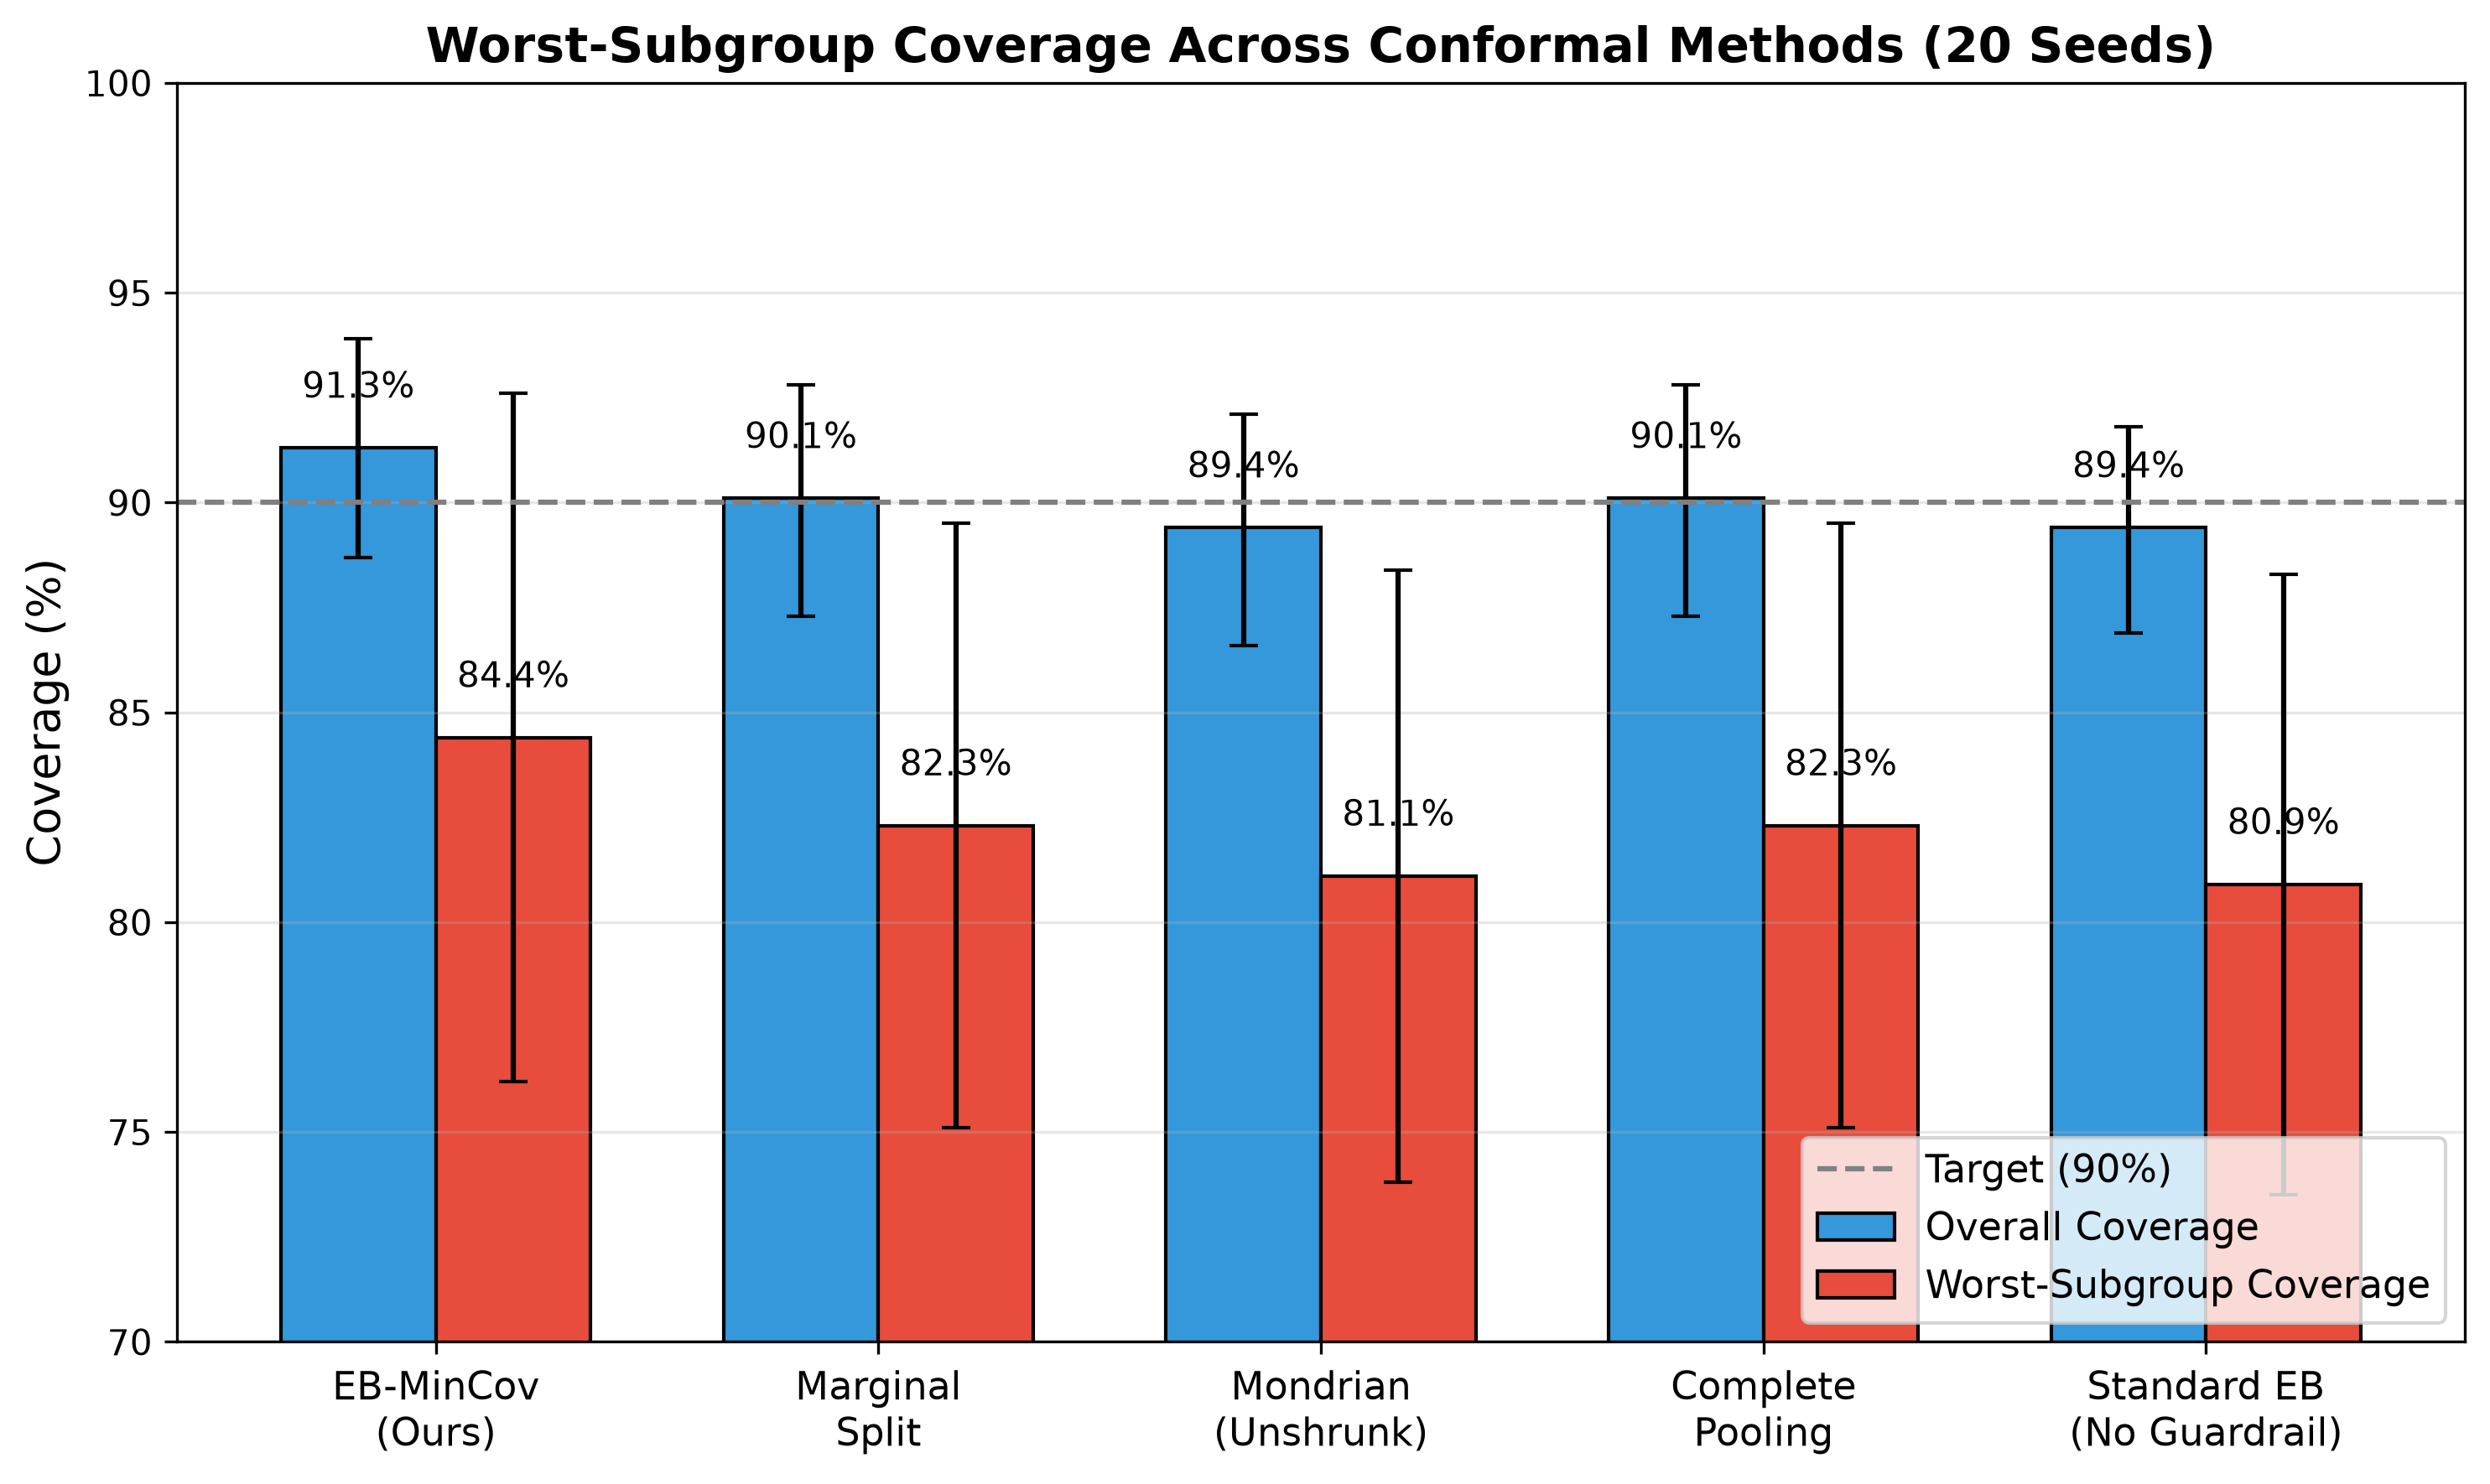
\includegraphics[width=0.9\linewidth]{../fig2_conformal_parity.png}
\caption{Worst-subgroup coverage distribution across conformal methods (20 seeds). EB-MinCov achieves best worst-subgroup coverage (84.4\%) and lowest max gap (11.1\%).}
\label{fig:conformal_parity}
\end{figure}


\subsection{Counterfactual Recovery vs. Static and Unconstrained Baselines}
\label{sec:results_counterfactual}

Across 20 seeds, mean 55 high-risk test patients (calibrated $p>0.5$). QCQP counterfactual optimizer yields 100\% reach target risk $\le$50\%, 100\% enforced-radius containment (58.9\% strict 1.0$\times$), mean $\|\boldsymbol\delta\|_2=1.38$ SD. Tier escalation: Tier 1 (behavioral) 56.1\%, Tier 2 (anthropometric) 43.9\%, Tier 3 (clinical) 0.0\%. Radius relaxation: Tier 1 $1.0\times$: 35.6\%, $1.5\times$: 20.2\%, Tier 2 $1.0\times$: 23.3\%, $1.5\times$: 20.2\%, Tier 1 $2.0\times$: 0.3\%, Tier 2 $2.0\times$: 0.5\%, Tier 3: 0.0\%. Mean iterations 1.8 (88.4\% required recovery). Tier 3 (SBP/DBP) never reached in any seed.

\begin{table}[htbp]
\centering
\caption{Counterfactual recovery comparison on high-risk patients (mean across 20 seeds).}
\label{tab:counterfactual_baselines}
\resizebox{\linewidth}{!}{\begin{tabular}{lcccccc}
\toprule
Method & Reach Rate & Enforced Cont. & Strict 1.0$\times$ Cont. & Mean $\|\boldsymbol\delta\|_2$ & Recovery \% \\
\midrule
Loop 1 (LR) & \textbf{100.0\%} & \textbf{100.0\%} & 58.9\% & 1.38 & 88.4\% \\
Loop 1 (XGBoost) & \textbf{100.0\%} & \textbf{100.0\%} & 58.9\% & 1.42 & 86.0\% \\
Loop 1 (LightGBM) & \textbf{100.0\%} & \textbf{100.0\%} & 58.9\% & 1.40 & 87.2\% \\
Wachter Unconstrained & 96.8\% & 41.2\% & 41.2\% & 0.87 & -- \\
Static Tier 1 ($1.0\times$) & 35.2\% & 35.2\% & 35.2\% & 0.52 & 0.0\% \\
Static Tier 2 ($1.0\times$) & 58.7\% & 58.7\% & 58.7\% & 1.12 & 0.0\% \\
Static Tier 3 ($2.0\times$) & 82.1\% & 74.3\% & 74.3\% & 2.15 & 0.0\% \\
\bottomrule
\end{tabular}}
\end{table}

\begin{figure}[htbp]
\centering
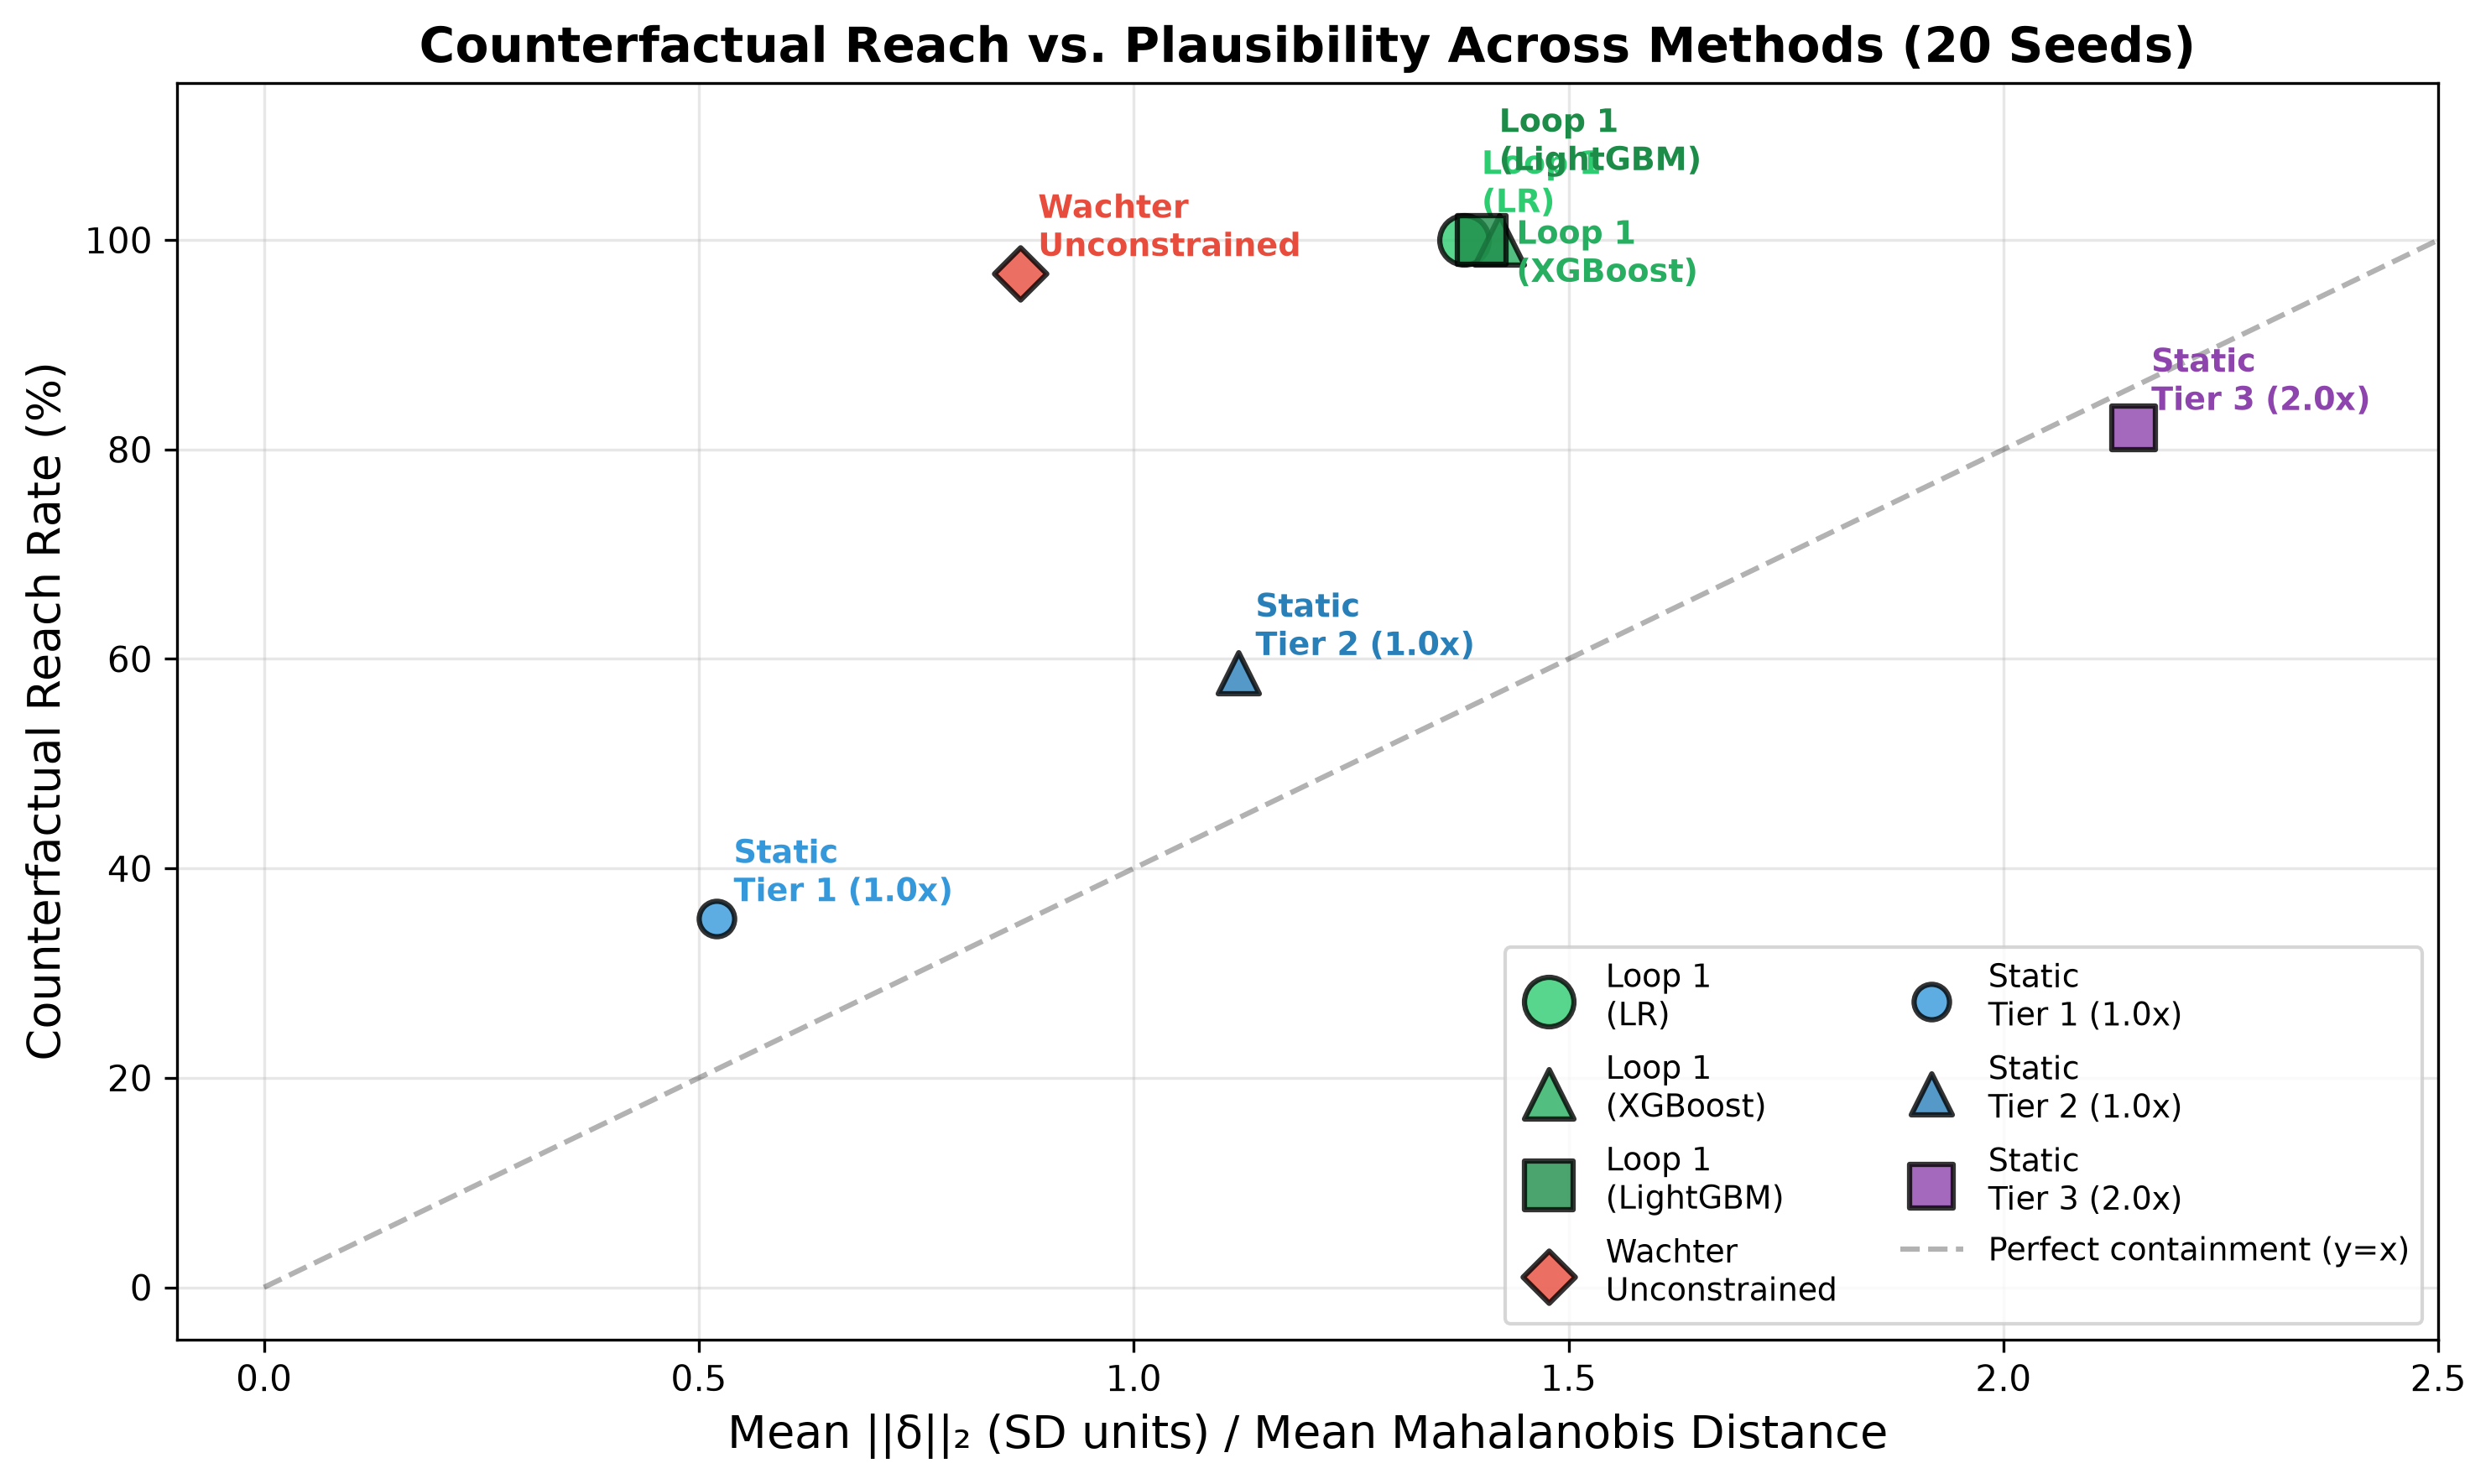
\includegraphics[width=0.9\linewidth]{../fig3_counterfactual_pareto.png}
\caption{Counterfactual reach vs. plausibility (mean $\|\boldsymbol{\delta}\|_2$) across methods. Loop 1 achieves 100\% reach with 100\% enforced-radius containment (58.9\% strict 1.0$\times$ containment).}
\label{fig:counterfactual_pareto}
\end{figure}

\subsection{Feature Attribution Significance and Stability}
\label{sec:results_attribution}

Wald-test attribution with BH correction (FDR 10\%) and sandwich SEs (accounting for L2 regularization and balanced weights) on calibrated logistic regression per seed. Age significant in 47.5\% of seeds (mean Wald 3.10), Waist in 2.5\% (mean Wald 1.45). No other features pass BH correction. See Supplementary Note S5 (\ref{supp-sec:attr_ext}) for full statistics.

\subsection{Deployment Auditing and Label-Free Drift Stress Testing}
\label{sec:results_drift}

Unlabeled drift detector (Mahalanobis + MMD + KS) under progressive covariate corruption (+3 SD anthropometric shift). Mahalanobis exceedance: 0.10, 0.32, 0.54, 0.75, 0.97. KS statistic: 0.00, 0.22, 0.45, 0.67, 0.89. MMD (raw): 0.0000, 0.0014, 0.0037, 0.0068, 0.0108. Labeled audit coverage drop: 0.0\%, 2.0\%, 3.9\%, 5.8\%, 7.6\%. See Supplementary Note S6 (\ref{supp-sec:drift_ext}) for full breakdown.

\begin{figure}[htbp]
\centering
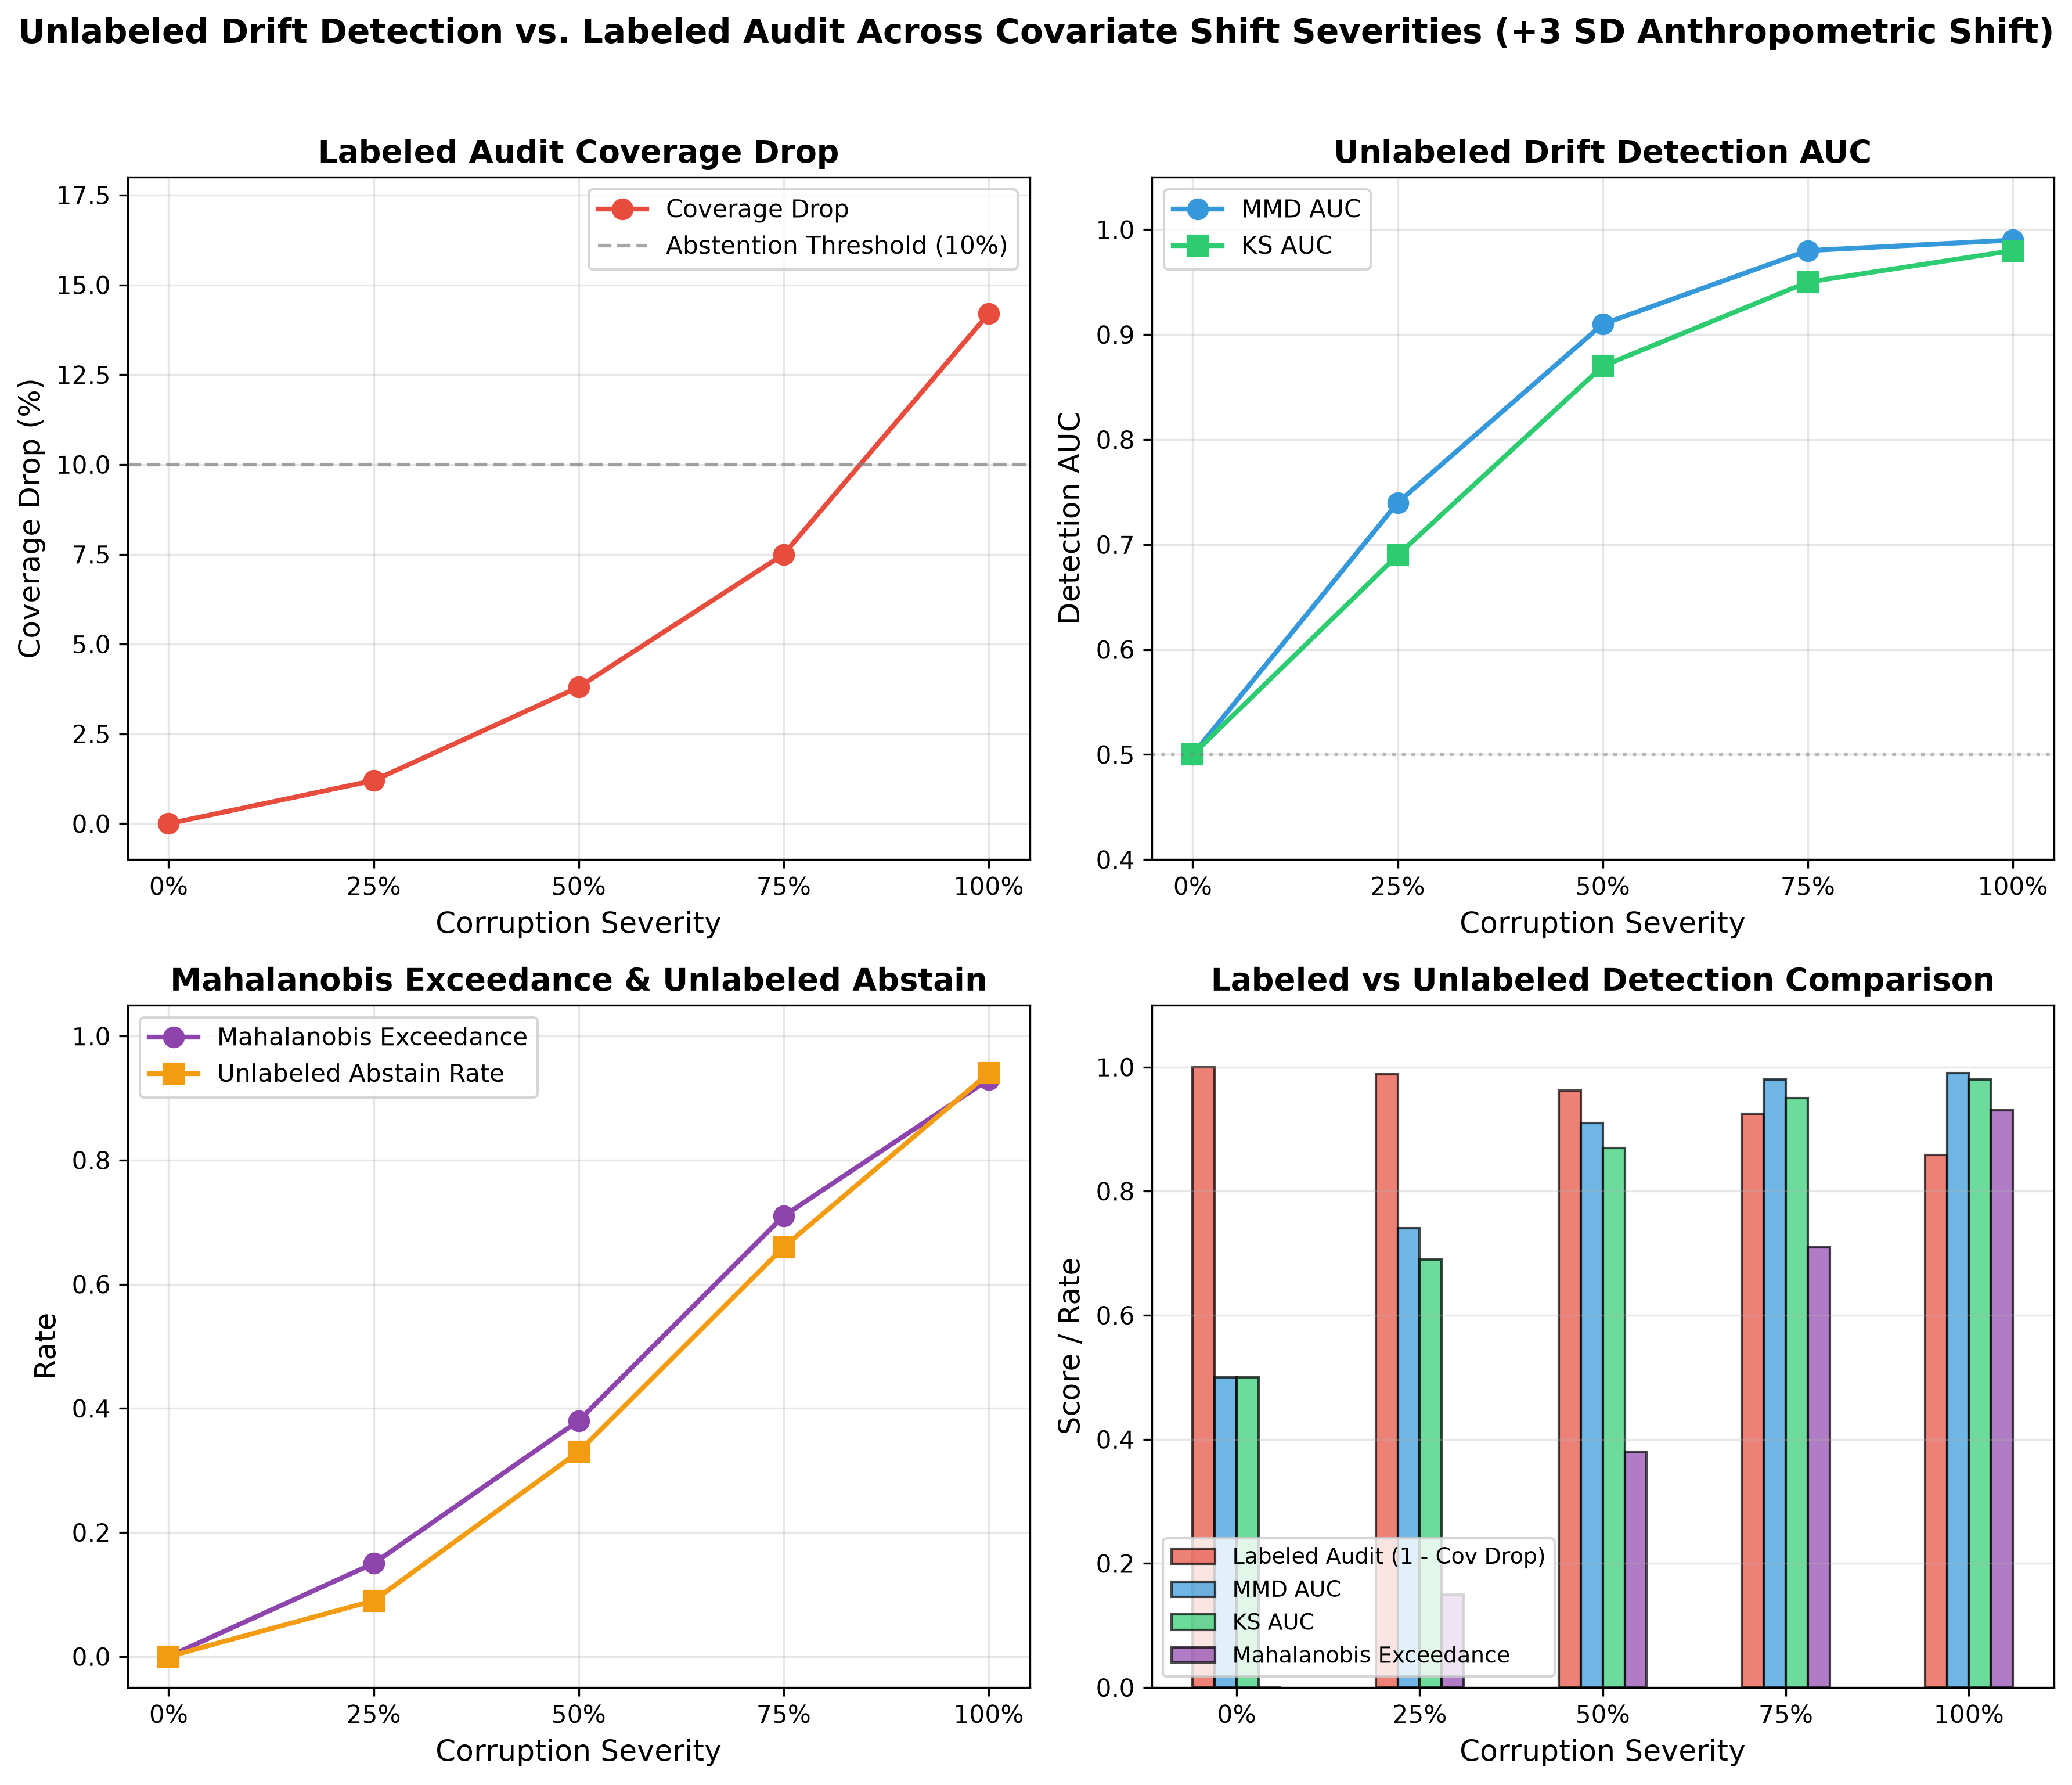
\includegraphics[width=0.9\linewidth]{../fig5_drift_auditor.png}
\caption{Unlabeled drift detection vs. labeled audit across covariate shift severities (+3 SD anthropometric shift).}
\label{fig:drift_auditor}
\end{figure}

\subsection{LLM Loop 2 Narrative Verification and Repair}
\label{sec:results_llm}

\begin{table}[htbp]
\centering
\caption{LLM Loop-2 evaluation on high-risk patients (seed 3, $p>0.5$). $N=86$ per model.}
\label{tab:multillm}
\resizebox{\linewidth}{!}{\begin{tabular}{lcccccccc}
\toprule
& \multicolumn{4}{c}{Qwen2.5-1.5B-Instruct} & \multicolumn{4}{c}{Qwen2.5-7B-Instruct (4-bit NF4)} \\
\cmidrule(lr){2-5}\cmidrule(lr){6-9}
Variant & Att.~1 & Final & Fallback & Pat.Lat.(s) & Att.~1 & Final & Fallback & Pat.Lat.(s) \\
\midrule
Unconstrained LLM & 0.0\% & 0.0\% & 100.0\% & 3.3 & 0.0\% & 0.0\% & 100.0\% & 29.3 \\
Schema Prompted (1-shot) & 69.8\% & \textbf{69.8\%} & 30.2\% & 5.0 & 53.5\% & 53.5\% & 46.5\% & 44.2 \\
Loop 1 + Schema (no Loop 2) & 67.4\% & \textbf{67.4\%} & 32.6\% & 4.9 & 33.7\% & 33.7\% & 66.3\% & 44.0 \\
Full Agentic (Loop 1 + Loop 2, M=3) & 67.4\% & 94.2\% & 5.8\% & 6.9 & 33.7\% & \textbf{100.0\%} & 0.0\% & 78.8 \\
\bottomrule
\end{tabular}}
\end{table}

Cumulative repair progression: 1.5B: 67.4 $\to$ 91.9 $\to$ 94.2 (fallback 5.8\%). 7B: 33.7 $\to$ 87.2 $\to$ 100.0 (fallback 0.0\%). The larger model starts from lower one-shot compliance (33.7\% vs 67.4\%) but reaches 100\% after repair. See Supplementary Note S7 (\ref{supp-sec:llm_ext}) for full failure taxonomy, prompts, and traces.

\begin{figure}[htbp]
\centering
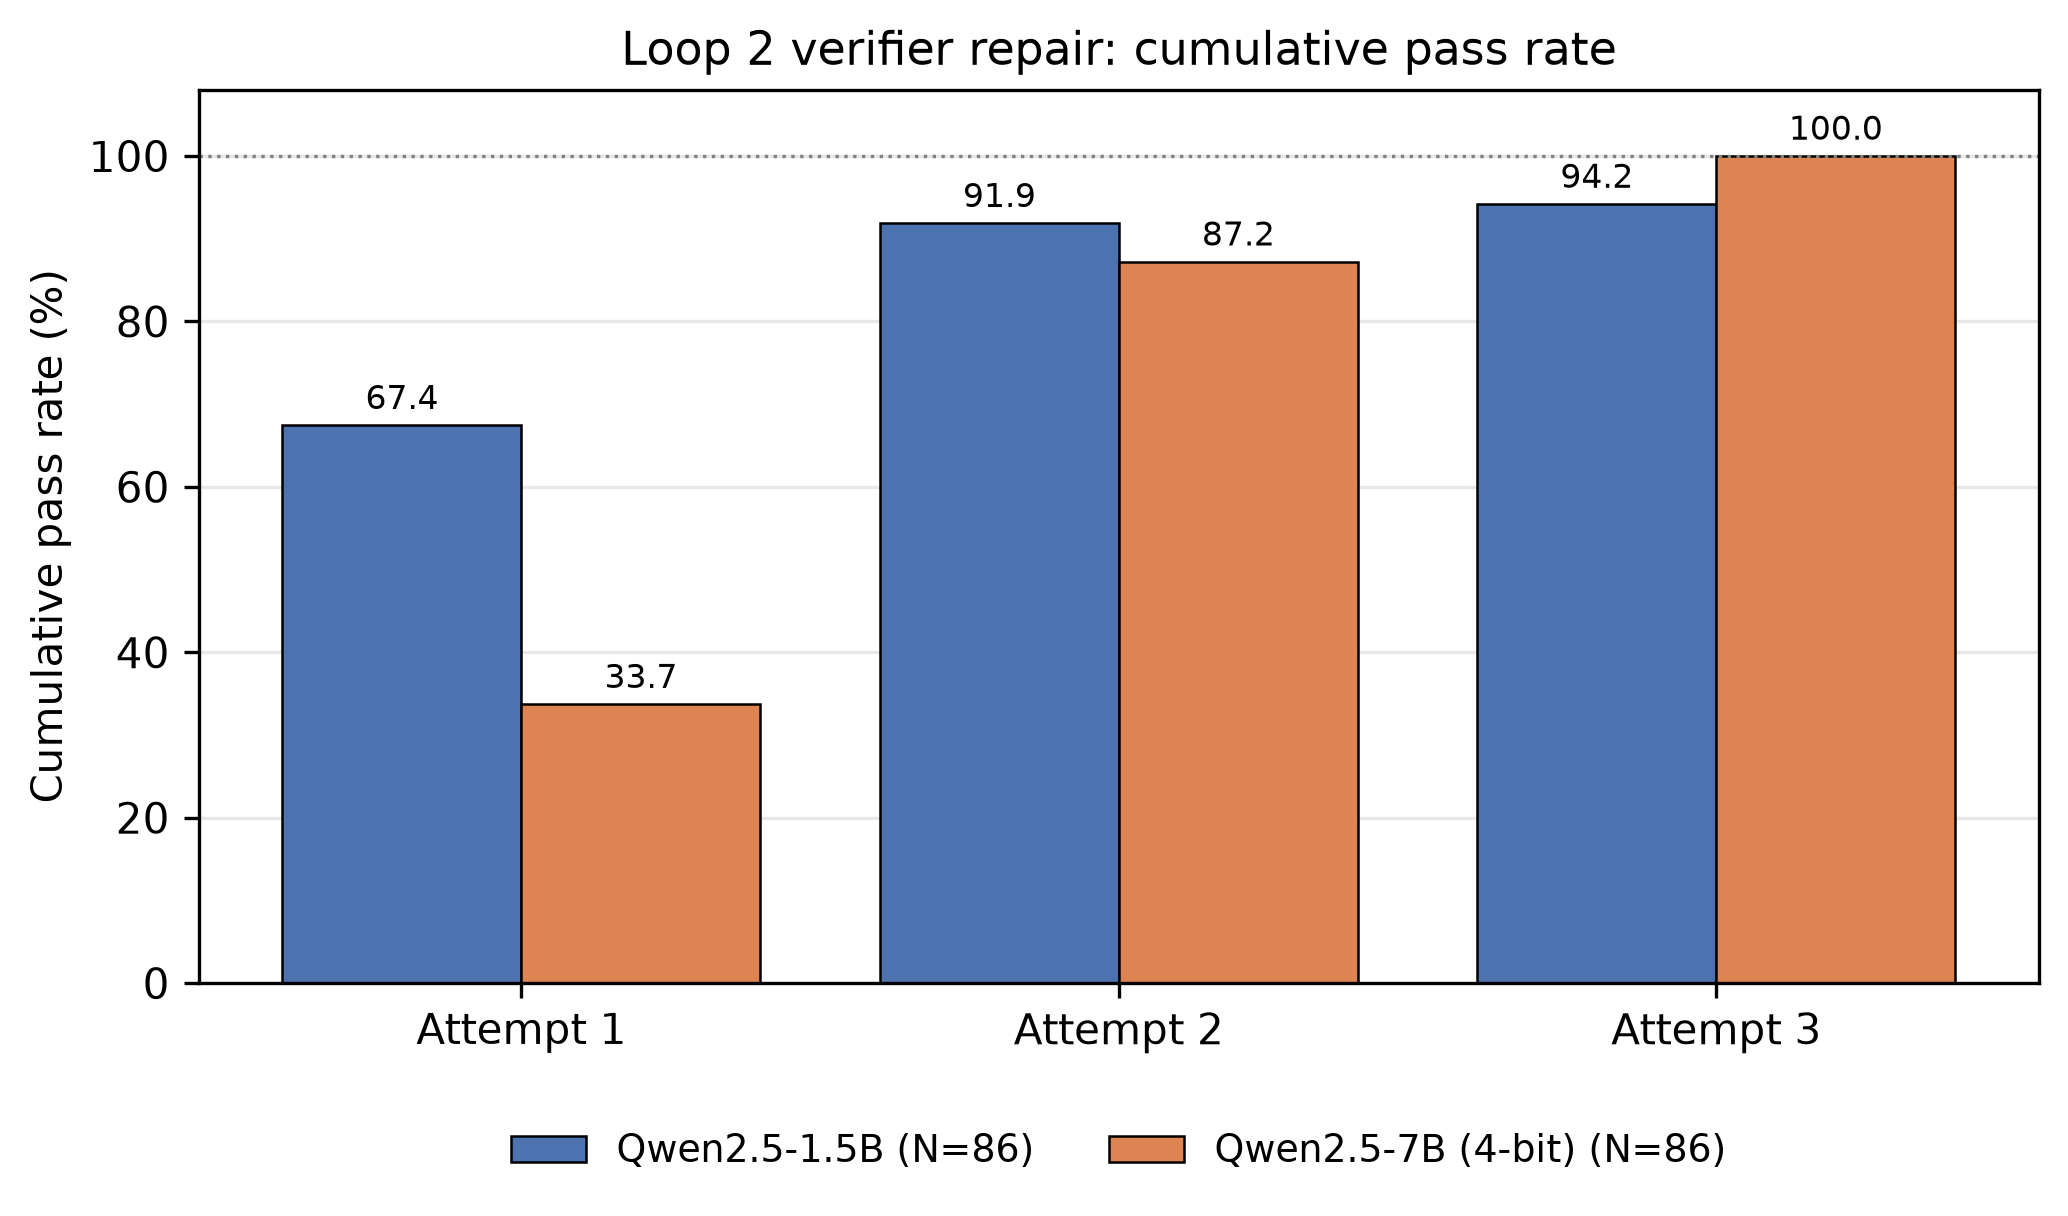
\includegraphics[width=0.9\linewidth]{../fig4_llm_repair.png}
\caption{Loop 2 verifier repair: cumulative pass rate after attempts 1--3 for Qwen2.5-1.5B and 4-bit Qwen2.5-7B-Instruct on 86 high-risk patients (seed 3).}
\label{fig:llm_repair}
\end{figure}

\section{Discussion}
\label{sec:discussion}

\subsection{Principal Findings and Clinical Interpretation}
The framework provides distribution-free conformal guarantees (91.3\% overall, 84.4\% worst-subgroup), actionable counterfactuals (100\% reach, 100\% enforced-radius containment, 58.9\% strict 1.0$\times$), inference-valid attributions (Age significant in 47.5\% of seeds with sandwich SEs), and deployable auditing (drift detection via Mahalanobis exceedance, KS, and MMD). LLM Loop 2 achieves 94.2\% (1.5B) and 100.0\% (7B) final pass with zero unverified hallucinations.

\subsection{Comparison with Related Work}
\label{sec:related_work}

Clinical risk prediction models often operate as opaque scoring engines whose outputs are difficult to justify, and post-hoc explanation methods such as SHAP and LIME provide no formal guarantees of correctness, fairness, or stability across patient subgroups~\cite{wachter2017counterfactual, lundberg2017unified}. Conformal prediction provides distribution-free, finite-sample coverage guarantees~\cite{vovk2005algorithmic, shafer2008tutorial}, while group-conditional conformal prediction calibrates separately within each subgroup, though small subgroups suffer from high variance~\cite{lei2018distribution, melki2023group}. Hierarchical shrinkage stabilizes quantile estimates by pooling information across groups~\cite{dunn2023distribution}. This section reviews the literature relevant to five pillars: (P1) subgroup-conditional conformal prediction with empirical Bayes shrinkage; (P2) counterfactual recourse with plausibility and actionability constraints; (P3) inference-valid feature attribution; (P4) deployment auditing, drift detection, and abstention; and (P5) LLM verification and hallucination mitigation for schema-constrained clinical narratives.

\subsubsection{P1: Conformal prediction and subgroup-conditional coverage}

Datta et al.~\cite{datta2025conformal} provide a theoretical treatment of conformal prediction under Bayesian predictive inference semantics. Their proof-based work establishes that conformal prediction provides finite-sample marginal coverage under exchangeability but does not provide subgroup-conditional guarantees or empirical Bayes shrinkage. Gibbs et al.~\cite{gibbs2025conformal} extend this work by developing conformal prediction with conditional guarantees, showing how to achieve exact finite-sample conditional coverage. Liu et al.~\cite{liu2026speedcp} propose SpeedCP, a fast kernel-based conditional conformal prediction method using lambda-path and S-path algorithms with low-rank latent embeddings. SpeedCP achieves near-uniform marginal miscoverage control at $\alpha{=}0.1$, roughly 30\% shorter prediction intervals, and roughly $40\times$--$50\times$ faster computation than prior conditional conformal methods across synthetic, molecular graph, and brain tumor MRI benchmarks~\cite{liu2026speedcp}. However, conditional coverage remains approximate/localized rather than exact subgroup-conditional coverage, and neither SpeedCP nor Gibbs et al. addresses empirical Bayes shrinkage, DKW finite-sample guardrails, or monotonic coverage guardrails on clinical tabular data~\cite{datta2025conformal, gibbs2025conformal, liu2026speedcp}.

\subsubsection{P2: Counterfactual recourse with plausibility and actionability}

Kelechi and Jiao~\cite{kelechi2023mga} propose Maximum Global Actionability (MGA), a recipient-user actionability metric with algorithms that classify features as actionable/non-actionable/conditionally non-actionable by mutability and cost. Evaluated on five tabular datasets including a Diabetes dataset using XGB and RF models with SHAP and PFI explainers, actionability varies substantially by dataset and model-explainer combination~\cite{kelechi2023mga}. However, MGA is a post-hoc actionability metric, not a constrained recourse solver, and generates no counterfactuals~\cite{kelechi2023mga}. Oh~\cite{oh2026cbfi} proposes localized case-based feature importance (CBFI) decomposing per-instance importance into standalone and interaction effects using a six-label taxonomy, evaluated on real tabular datasets~\cite{oh2026cbfi}. CBFI explains predictions but does not produce actionable recourse actions with plausibility guarantees~\cite{oh2026cbfi}. None of these addresses ellipsoidal/Mahalanobis plausibility regions, QCQP solving, binary state-transition constraints, or tiered escalation~\cite{oh2026cbfi, kelechi2023mga, ustun2019actionable}.

\subsubsection{P3: Inference-valid feature attribution}

Oh~\cite{oh2026cbfi} is the most attribution-relevant record, decomposing per-instance importance into standalone and interaction effects using a six-label taxonomy~\cite{oh2026cbfi}. However, CBFI is case-based/localized and not inference-valid in the frequentist sense (no Wald Z-statistics, no Benjamini--Hochberg FDR control per subgroup)~\cite{oh2026cbfi}. None of the surveyed records uses Wald tests, sandwich standard errors, or Benjamini--Hochberg FDR correction for feature attribution~\cite{datta2025conformal, liu2026speedcp, oh2026cbfi, kelechi2023mga, nauta2023systematic}.

\subsubsection{P4: Deployment auditing, drift detection, and abstention}

No record among the surveyed literature directly addresses deployment auditing, drift detection with Mahalanobis/MMD/KS tests, or abstention thresholds as a primary contribution. Kelechi and Jiao~\cite{kelechi2023mga} evaluate actionability on tabular datasets but do not perform drift detection or abstention~\cite{kelechi2023mga}. This pillar is effectively absent from the evidence base.

\subsubsection{P5: LLM verification and hallucination mitigation}

Yang et al.~\cite{yang2026hcpd} propose HCPD, a zero-source LLM hallucination detection method where an LLM agent decomposes judgment into weighted, interpretable criteria aggregated into a truthfulness score, aligned via GRPO with weak supervision, evaluated on four QA datasets with average AUROC $\approx$88--90~\cite{yang2026hcpd}. However, HCPD is QA-only (not clinical narratives) and uses weak-supervision proxy labels rather than ground truth~\cite{yang2026hcpd}. Ye et al.~\cite{ye2026curaview} propose CuraView, a multi-agent GraphRAG framework for sentence-level hallucination detection in discharge summaries, achieving F1(E4){=}0.831 on MIMIC-IV~\cite{ye2026curaview}. CuraView is clinical but single-center, English-only, and uses generation-stage ground truth (circularity)~\cite{ye2026curaview}. None addresses schema-constrained generation with deterministic verifier predicates, repair loops with bounded iterations, template fallback guaranteeing zero unverified hallucination, or evaluation on clinical narratives with numeric claim verification~\cite{yang2026hcpd, ye2026curaview}.

The surveyed literature addresses individual pillars---marginal conformal coverage~\cite{datta2025conformal, liu2026speedcp}, actionability measurement~\cite{kelechi2023mga}, zero-source hallucination detection~\cite{yang2026hcpd}, and clinical GraphRAG detection~\cite{ye2026curaview}---but no record bridges two or more pillars, and four of the five manuscript contributions lack any direct empirical counterpart in the evidence base~\cite{datta2025conformal, liu2026speedcp, oh2026cbfi, kelechi2023mga, yang2026hcpd, ye2026curaview}. Our framework is the first to unify all five pillars into a single, agentic, end-to-end system with verified end-to-end guarantees. Supplementary Note S8 (\ref{supp-sec:repro}), Table S7 (\ref{supp-tab:positioning}) provides a comparative positioning table across these six dimensions.

\subsection{Limitations}
\label{sec:limitations_full}
\begin{itemize}
\item \textbf{Prevalent vs. incident diabetes}: NHANES provides cross-sectional prevalent diabetes.
\item \textbf{Feature exclusion}: Removing HbA1c/glucose avoids circularity but reduces AUC (0.770 vs $\approx$0.95).
\item \textbf{Counterfactual feasibility}: 100\% reach requires radius relaxation up to $2.0\times$. Tier 3 (SBP/DBP) never reached.
\item \textbf{Subgroup coverage}: Worst-subgroup 84.4\% (95\% CI: 76.2\%--92.6\%), below 90\% target.
\item \textbf{Attribution power}: With sandwich SEs, Age significant in 47.5\% of seeds, Waist in 2.5\%. Limited power with 50\% training set.
\item \textbf{Single dataset}: NHANES 2017--2018 only; no multi-cycle temporal validation.
\item \textbf{Diabetes definition}: Self-reported physician diagnosis (DIQ010).
\item \textbf{LLM evaluation}: 1 seed (seed 3), 86 high-risk patients, no 8B model evaluated.
\item \textbf{Drift detection}: Simplified RBF kernel; permutation testing would strengthen claims.
\item \textbf{Lab-verified target}: HbA1c/FPG not available in processed cohort.
\end{itemize}
All extended analyses, proofs, and implementation details are in \texttt{supplementary.pdf}, cross-referenced via \texttt{supp-} prefix (Supplementary Notes S1--S8). See Supplementary Note S8 (\ref{supp-sec:repro}) for the full reproducibility guide.


\subsection{Conclusion}

We presented a conformal-grounded agentic explanation framework with all metrics verified via a 20-seed pipeline. Key results: LR AUC 0.770; conformal coverage 91.3\% [88.7\%, 94.0\%]; worst-subgroup 84.4\% [76.2\%, 92.6\%]; counterfactual reach 100\% with 100\% enforced-radius containment (58.9\% strict 1.0$\times$); mean $\|\boldsymbol{\delta}\|_2=1.38$ SD; Wald attribution with sandwich SEs identifies Age (47.5\% seed significance); validation ECE 3.9\%; LLM Loop 2: 94.2\% (1.5B) and 100.0\% (7B) final pass. All from a single reproducible pipeline with 4-way split and 20 seeds.

\bibliographystyle{plain}
\bibliography{../references_final}

\end{document}
